The internal structure of jets in the forward region were examined using 2010 data to assess how well the MC simulation reproduces the data.
The transverse size of the jet is quantified using the jet width,
\begin{equation}
\mathrm{Width}=\frac{\sum (r^{\mathrm{cluster}} \times \et{}^{\mathrm{cluster}}) }{\sum \et{}^{\mathrm{cluster}}},
\label{JetPerf:Width}
\end{equation}
where the sums are over all clusters within the jet, and $r^{\mathrm{cluster}}$ is the distance of each cluster from the jet centre.
Another important jet observable is the electromagnetic fraction (EMF), which is the fraction of the total jet energy (at EM scale) coming from electromagnetic clusters.


Figure \ref{JetPerf:Width_EMF} (a) shows the jet width for jets in the forward region.
Figure \ref{JetPerf:Width_EMF} (b) shows the EMF for jets in the forward region.
The data are compared to PYTHIA using three different physics lists which use different calorimeter interaction models.
The three physics lists used, QGSP, $\rm QGSP\_BERT$, and $\rm FTFP\_BERT$ are discussed in \cite{ref:HadModels}. 
These lists define different aspects of modelling the interactions of hadrons with matter and are shown in Table \ref{JetPerf:Models}.

The QGSP \cite{ref:QGSPNew} physics list contains the quark gluon string model, which is a phenomenological model describing the parton production arising from collisions between hadrons and nucleons, for high energy hadrons, and uses a low energy parameterisation model (LEP), which is based on extrapolating measured reaction cross-sections for the low energy hadrons.  
The $\rm{QGSP\_BERT}$ physics list still uses QGSP at high hadronic energy, but only uses LEP at medium energies.
For low energy hadrons, the Bertini nucleon-nucleon scattering model (BERT) \cite{ref:BERTNew} is used. This is an alternative model for the low energy interaction of hadrons in  the nucleon medium.
$\rm{FTFP\_BERT}$ uses the  Fritiof fragmentation model (FTF) \cite{ref:FTFNew} to model the high energy interactions. 
In regions where there is overlap between the different models, there is linear interpolation between them.


By comparing the standard PYTHIA physics list, $\rm QGSP\_BERT$, to QGSP and $\rm FTFP\_BERT$, the effects of removing the BERT model and also changing from the QGS model to the FTF model can be seen.

\begin{table}
\centering
\begin{tabular}{ | c | c | c | c |}
\hline
\hline
Physics List& \multicolumn{3}{ c |}{Hadron Energy Range (GeV)} \\ 
& Low & Medium & High \\ 
\hline
           QGSP    &                       &    $0-25$ LEP     &    $>12$ QGSP \\
$\rm QGSP\_BERT$   &    $0-9.9$ BERT   &    $9.5-25$ LEP   &    $>12$ QGSP \\
$\rm FTFP\_BERT$   &    $0-5$ BERT     &                   &    $>4$ FTF   \\
\hline
\hline
\end{tabular}
\caption[Physics lists description of hadron interaction models used for various hadron energies]{
Hadron interaction models for different physics list for various hadron energies.
Taken from Table 6 in \cite{ref:HadModels}.
\label{JetPerf:Models}}
\end{table}

None of the physics lists manage to accurately describe the data, and the width is consistently higher in data than in the simulations. 
These differences have also been observed for central jets, though with smaller magnitude \cite{ref:JetShapes}.
As concluded in \cite{ref:HadModels}, the physics lists chosen as default at ATLAS produced narrower and shorter showers than data, but gave the best agreement with the data for the pion response.
These results have been published in an ATLAS conference note~\cite{ref:EtaInter2010}. 

\begin{figure}
\centering
        \begin{subfigure}[b]{0.5\textwidth}
                \centering
                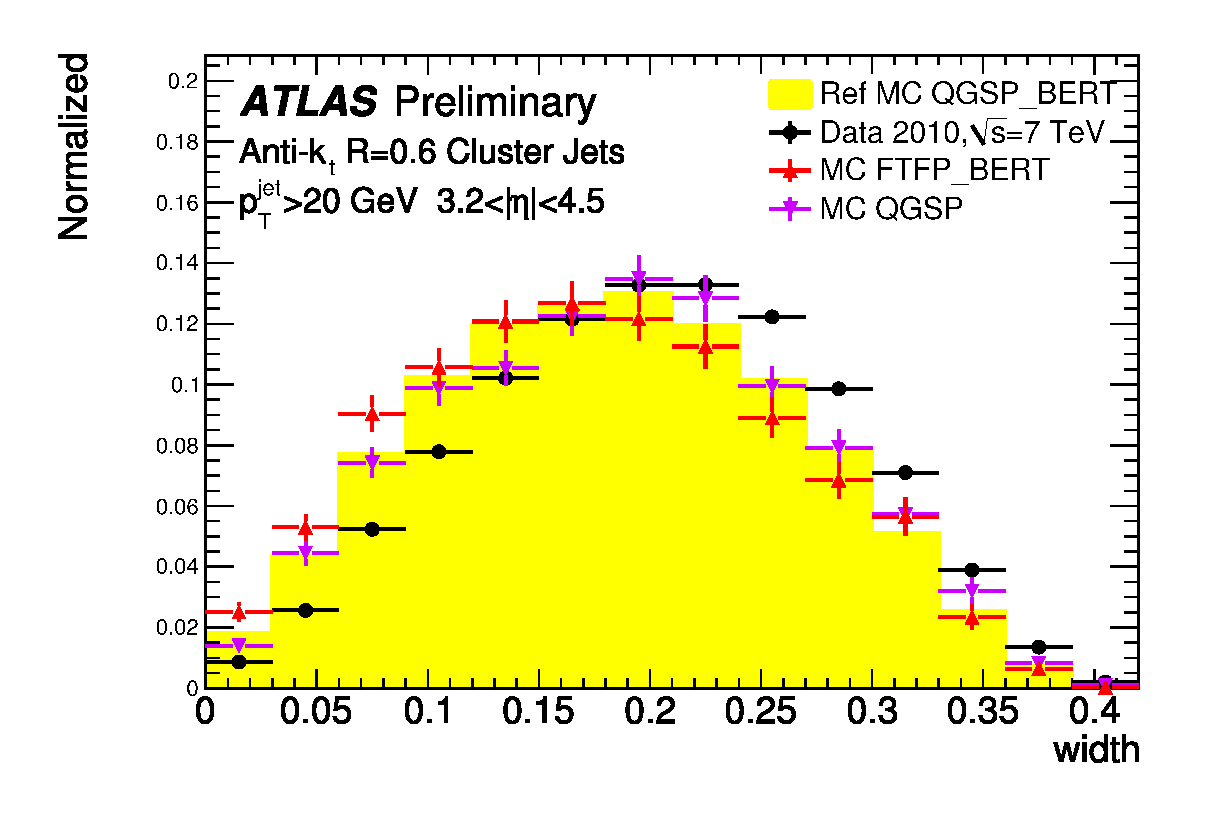
\includegraphics[width=\textwidth]{figures/JetPerformance/Width.eps}
        \end{subfigure}%
        \begin{subfigure}[b]{0.5\textwidth}
                \centering
                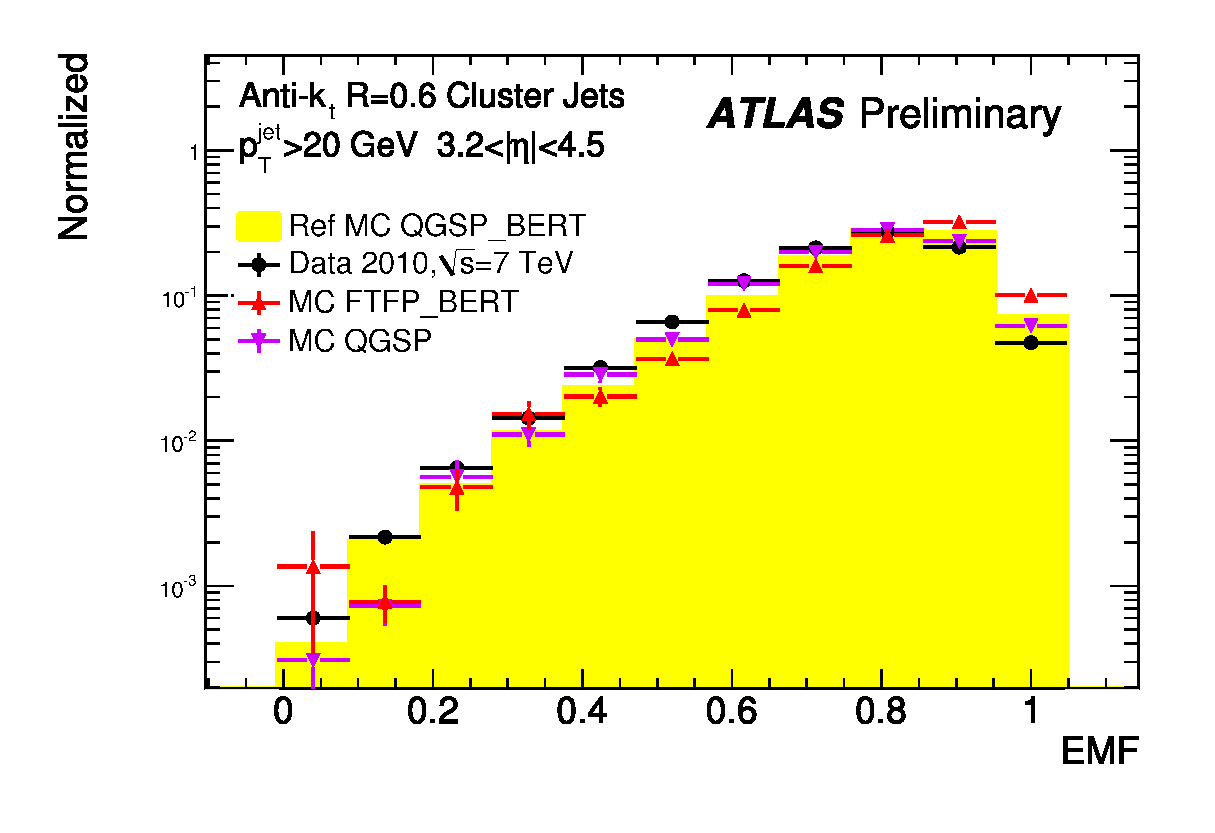
\includegraphics[width=\textwidth]{figures/JetPerformance/EMF.eps}
        \end{subfigure}%
\caption[Comparison of jet widths and EMF for data compared to PYTHIA with various physics lists]{
(a) Jet width and (b) jet EMF for jets with \pt{}$>20$ GeV and in the region \etaRange{3.2}{4.5}.
2010 data is compared to standard PYTHIA with the different physics lists, $\rm QGSP\textunderscore{}BERT$ (yellow filled), $\rm FTFP\textunderscore{}BERT$ (red circles) and $\rm QGSP$ (purple circles).  
\label{JetPerf:Width_EMF}}
\end{figure}

